\section{Použití - oděvy, rukavice a obuv}

\begin{frame}
	\frametitle{Důvod}
	\begin{itemize}
		\item Nedostatečná nabídka voděodolných a zároveň prodyšných materiálů
		\item Původně určená pouze pro oděvy a stany
		\item Patent podán roku 1978 (US 4194041 A)
	\end{itemize}
\end{frame}

\begin{frame}
	\frametitle{Oděvy, rukavice a boty}
	\begin{itemize}
		\item Myšlenka materiálu: udržet vodu venku a zároveň nechat projít ven vlhkost
		\item Gore-Tex\textregistered nabízí 4 varianty konstrukce tkanin pro oděvy
		\begin{itemize}
			\item 2 vrstvá konstrukce % Out+gore, inner
			\item 3 vrstvá konstrukce % Out+gore+inner
			\item Z-liner konstrukce % Out, gore, inner
			\item LTD konstrukce % Out, gore+inner
		\end{itemize}
	  	\item V těchto konstrukcích se vyrábí kalohty a bundy.
	  	\item Rukavice mají navíc ještě tepelnou izolaci.
	\end{itemize}
\end{frame}

\begin{frame}
	\frametitle{2 vrstvá konstrukce}
			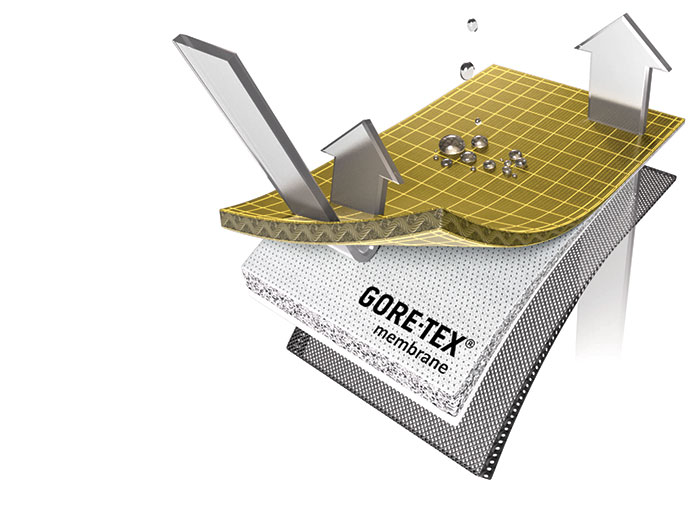
\includegraphics[width=0.8\textwidth]{bunda_close.jpg}
		\zdroj{http://www.gore-tex.com/en-us/technology/outerwear/gore-tex-products}
\end{frame}

\begin{frame}
	\frametitle{Konstrukce obuvi}
	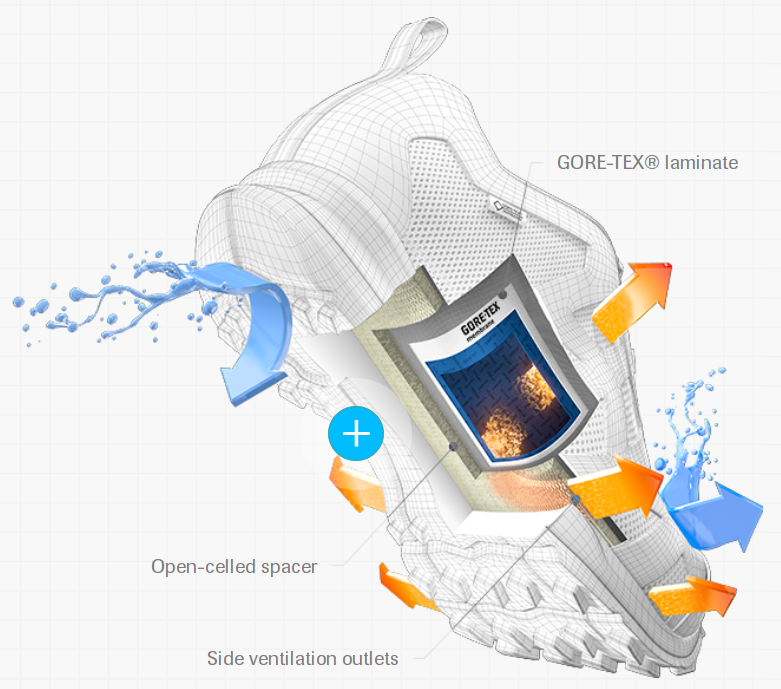
\includegraphics[width=0.65\textwidth]{bota_close.png}
	\zdroj{http://www.gore-tex.com/en-us/technology/footwear/gore-tex-surround-outdoor-footwear}
\end{frame}
